\section{Introduction}

This section gives an overview about the reasoning behind the creation of this 
thesis, along with a comparison of similar studies. For a practically oriented overview of this thesis, refer to Figure~\ref{fig:graphical_overview}.

\subsection{Motivation}

Cancer is one of the leading causes of death in adults worldwide. Estimated to
be the third most diagnosed type of cancer in 2020, colorectal cancer is both 
common and carries a high mortality rate~\cite{cancer_stats_2020}. The response to treatment varies 
between patients, where complete recovery is known as \acf{pcr}~\cite{Zorcolo2012}.
The prediction of \ac{pcr} aides in the choice of treatment of patients suffering
from tumors~\cite{radiomics_analysis_pcr_rectal}. Although this prediction has 
been the aim multiple studies, the methodology used is often difficult to 
reproduce, through the use of either undocumented or non-standard
implementations. 

\subsection{Aim of this Thesis}

The aim of this thesis is to investigate a connection between statistical 
features of common \ac{mri} images and the \ac{pcr} of a patient.
A radiomics-based
machine learning model in the shape of \iac{rf}-based classifier, will be used 
in an attempt to predict \ac{pcr} in 
colorectal tumor patients significantly better than trough random choice.
To improve reproducibility, publicly accessible and well-document tools will be 
used. Where applicable, the idea behind custom implementations and their mode
of operation shall be well-described, in order to be easily replicated.


\subsection{State of Research}\label{sec:state_of_research}

Numerous papers have been written about the analysis of tumors using radiomics,
though the focus on colorectal tumors is comparatively sparse. As of time of 
writing, three other papers are known to focus on the prediction 
of \ac{pcr} via radiomics features extracted from \ac{mri} scans of rectal 
tumors~\cite{radiomics_analysis_pcr_rectal,rectal_radiomics_svm_rf,multisite_rectal_radiomics}.
A comparison of methodology and results of these studies is shown in 
Table~\ref{tbl:other_studies_auc}. All three studies were successful in 
separating \ac{pcr} and non-\ac{pcr} patients at a rate better than through 
simple guesses. Two of these studies employed either \iac{rf}-based model, or
one including \iac{rf} classifier.

\begin{table}[H]
    \centering
    \begin{tabular}{c c c c c}
        Study & Patients in Dataset & Classification Model & AUC & \SI{95}{\percent} Confidence Interval \\
        \hline
        \cite{radiomics_analysis_pcr_rectal} & \num{222} & \acs{svm} & \num{0.9756} & [\num{0.9185}, \num{0.9711}] \\
        \cite{rectal_radiomics_svm_rf} & \num{134} & Mixed, including \acs{svm} and \acs{rf} & \num{0.91} & [\num{0.83}, \num{0.98}] \\
        \cite{multisite_rectal_radiomics} & \num{104} & \acs{rf} & \num{0.712} & --- % TODO: Check if Hold-out of Discovery validation should be used TODO: What is the confidence interval?
    \end{tabular}
    \caption{A comparison of studies on the prediction of \ac{pcr} using \ac{mri}-based radiomics features. Where missing, data was not available from the original study.}\label{tbl:other_studies_auc}
\end{table}

Although all datasets
consisted of \ac{mri} imaging data, significant differences in scan 
composition were shown. All studies included T\textsubscript{2} weighted scans, 
with~\cite{radiomics_analysis_pcr_rectal} using additional \ac{dwi} data, where each weighting was recorded at 
two distinct points in time.~\cite{rectal_radiomics_svm_rf} states access to
additional T\textsubscript{1} weighted scans, though it focuses on the analysis 
of T\textsubscript{2} data.

Additionally, selection of \ac{roi} varied in methodology. While all studies 
used manual annotations, \cite{multisite_rectal_radiomics} utilized a combined 
approach of using both the largest available tumor slice and a volumetric 
representation of the entire tumor, while~\cite{rectal_radiomics_svm_rf} 
and~\cite{multisite_rectal_radiomics} opted for the former and latter approaches
respectively.

Although automated and semi-automatic tumor annotation techniques are in 
development, all studies listed in Table~\ref{tbl:other_studies_auc} opted for 
manual annotation. As non-manual annotation technologies are, as of time of 
writing, not clearly standardized, a simple \enquote{a priori} shape-based 
algorithm has been used to semi-automatically create 3-dimensional 
annotations in the context of this thesis~\cite{auto_and_semiauto,semiautomatic_prostate,dl_rectal_segmentation}.

For the extraction of radiomics features, both~\cite{radiomics_analysis_pcr_rectal}
and~\cite{multisite_rectal_radiomics} opted for differing custom implementations
using MATLAB\footnote{The MathWorks, Inc.}, where in both cases a description, 
of varying detail, of the features utilized, was published. In contrast,~\cite{rectal_radiomics_svm_rf} chose MaZda~\cite{mazda},
an image texture analysis toolkit. This shows the common intent of a transparent 
feature definition. Though this helps in increasing
reproducibility~\cite{ibsi_paper,radiomics_process_and_challenges}, two 
out of three studies used MATLAB for feature extraction, 
while~\cite{rectal_radiomics_svm_rf} later relies on MATLAB for classification.
This may hinder availability of the methods described in these studies, as 
MATLAB is, as of time of writing, commercial software~\cite{matlab}.
Additionally, even well-documented custom implementations of radiomics features pose 
problems for the comparison between studies, as addressed by~\cite{ibsi_paper}.
To alleviate problems associated with both inconsistent feature definitions and
the potential unavailability of commercial software, this thesis is based on an 
open-source radiomics library, which largely follows \ac{ibsi} recommendations
for feature definitions.

Although using different sets of features and feature definitions, all studies
shown use at least one common method of selecting features (\ac{lasso}~\cite{lasso}).
Additional commonality arises from the features selected, as feature groups
chosen by each study consist largely of texture-based features, such as 
\ac{collage} and Gray-Level Matrices~\cite{radiomics_analysis_pcr_rectal,rectal_radiomics_svm_rf,multisite_rectal_radiomics,collage}.

As the only known study to utilize an identical classifier setup (a purely 
\ac{rf}-based classifier) for the problem posed in this thesis (predicting \ac{pcr} 
in colorectal tumor patients),~\cite{multisite_rectal_radiomics} employs a 
combination of three feature selection variants. In contrast to these measures, 
a selection method based on the ability of \ac{rf} classifiers to determine the
contribution of individual features to the final classification performance is 
used. The choice of \iac{rf} classifier was based on the strength of such 
models to handle a large amount of features extracted from a relatively small 
sample size~\cite{random_forests_article,random_forests_web}. Indeed, the
number of patients in this study is consistently lower than all similar studies
referenced here (compare Section~\ref{sec:materials_dataset} and 
Table~\ref{tbl:other_studies_auc}).


% https://www.bu.edu/math/files/2013/08/tikzpgfmanual.pdf
% https://tex.stackexchange.com/questions/488983/tikz-style-for-rectangle-with-text-in-border
\begin{figure}[H]
    \centering
\begin{tikzpicture}[titlerect/.style={draw,inner ysep=2ex,inner
    xsep=1ex,minimum height = 2cm, minimum width={2*width("#1")},align=center,label={[anchor=center,fill=white,font=\Large]above:#1}}]


    \node (img_acq) [titlerect={Image Acquisition}] at (0,0) {\begin{tabular}{l r}
        Importance of Metadata & Section~\ref{sec:radiomics_image_acquisition} \\ 
        \acs{mri} & Section~\ref{sec:intro_mri}\\
        Dataset & Section~\ref{sec:materials_dataset}\\
        Metadata & Section~\ref{sec:mri_metadata} \\
    \end{tabular}};

    \node (img_seg) [below = of img_acq, titlerect={Image Segmentation}] {\begin{tabular}{l r}
        Concept & Section~\ref{sec:radiomics_image_segmentation} \\
        Annotation Extrapolation & Section~\ref{sec:3d_and_2d} \\
    \end{tabular}};

    \node (ftr_ext) [below = of img_seg, titlerect={Feature Extraction}] {\begin{tabular}{l r}
        Concept & Section~\ref{sec:radiomics_feature_extraction} \\
        Extraction & Section~\ref{sec:feature_extraction} \\
        Available Feature Groups & Section~\ref{sec:radiomics_features} \\
        Available Scan Filters & Section~\ref{sec:base_scan_filters} \\
        Configuration & Section~\ref{sec:pyrad_config} \\
    \end{tabular}};

    \node (ftr_als) [below = of ftr_ext, titlerect={Feature Analysis}] {
        \begin{tabular}{l r}
            Classifier & Section~\ref{sec:intro_classification} \\
            Experimental Setup & Section~\ref{sec:experimental_setup} \\
            Feature Selection & Section~\ref{sec:feature_filtering} \\
            Implementation & Section~\ref{sec:code_structure} \\
            \hline
        \end{tabular}

        \\

        \begin{tabular}{l r}
            \multicolumn{2}{c}{By Importance} \\
            Importance Assignment & Section~\ref{sec:filtering_importance} \\
        \end{tabular}
        \vline
        \begin{tabular}{l r}
            \multicolumn{2}{c}{By Grouping} \\
            Group Assignment & Section~\ref{sec:filtering_grouping} \\
        \end{tabular}
    };

    \node (eval) [below = of ftr_als, titlerect={Evaluation}] {
        \begin{tabular}{l r}
            Hypothesis & Section~\ref{sec:hypothesis}\\
            Results & Section~\ref{sec:results}\\
            Discussion & Section~\ref{sec:discussion}\\
        \end{tabular}
    };


    \draw [->, shorten <= 5pt, shorten >= 8pt] (img_acq.south) -- (img_seg.north);
    \draw [->, shorten <= 5pt, shorten >= 8pt] (img_seg.south) -- (ftr_ext.north);
    \draw [->, shorten <= 5pt, shorten >= 8pt] (ftr_ext.south) -- (ftr_als.north);
    \draw [->, shorten <= 5pt, shorten >= 8pt] (ftr_als.south) -- (eval.north);

\end{tikzpicture}
\caption{A rough overview of the sections that make up the central experiment this thesis covers. A summary of this setup is provided in Section~\ref{sec:experimental_setup}.}\label{fig:graphical_overview}
\end{figure}


\newpage{}
\section{Underlying Concepts}

This section gives an overview of concepts that form the base of this 
experimental setup. First, radiomics is described in more detail in 
Section~\ref{sec:intro_radiomics}, along with the imaging technology whose 
results it analyzes, which is examined in Section~\ref{sec:intro_mri}. Second, 
the classification model used here and its evaluation are covered in 
Section~\ref{sec:intro_classification}.

% Maybe break up these sentences^

% "Graphical Overview".
% Not sure how to structure this
% \begin{tikzpicture}[node distance=2cm]
%     \tikzstyle{startstop} = [rectangle, minimum width=3cm, minimum height=1cm,text centered, draw=black]
%     \node (concepts) [startstop] {Underlying Concepts};
% \end{tikzpicture}

\subsection{Radiomics}\label{sec:intro_radiomics}

% describe radiomics in more detail

Radiomics is an emerging field of study concerning the analysis of medical 
imaging data~\cite{applications_and_limitations_of_radiomics}. It aims to use
the products of widely used and available imaging technologies to extract 
additional information about a patient's health through statistical analysis.
It does so by the extraction of \textit{features}, discrete pieces of 
information describing an image's content, which later can be fed into a 
classifier model. Such features describe properties such as the shape of a tumor
inside a scan or the distributions of gray levels inside a specific area~\cite{radiomics_the_bridge,pcr_lymph,radiomics_process_and_challenges}.

For using radiomics as a base for classification, four steps are required; 
acquiring image data to be analyzed, marking \iac{roi} within those images, extracting 
radiomics features from an image and its newly generated \ac{roi}, and analyzing potential
interrelationships between the extracted features and expectations in a 
patient's development~\cite{radiomics_advanced_feature_analysis,radiomics_process_and_challenges}.
While these steps cover a rough outline of the entire radiomics workflow, some
authors may choose to further divide these steps into more detailed subroutines,
especially when focusing on one or more steps in particular 
(compare~\cite{ibsi_paper}).

\subsubsection{Image Acquisition}\label{sec:radiomics_image_acquisition}

% A number of technologies all have been developed to the same aim; to acquire an 
% image of a body, or body part to be examined. The non-invasive imaging methods 
% mentioned earlier have shown to be of special importance in analyzing 
% tumors~\cite{py_rad}. The specific method chosen here is \ac{mri}.

For images to be analyzed, these images must be present in the first place. This can
be accomplished any common or available medical imaging technology. The technology in focus here is \ac{mri}, the process of which is 
described in more detail in Section~\ref{sec:intro_mri}.

Though the focus of radiomics lies on the analysis of images 
themselves, metadata is not to be ignored. Imaging technologies generally are 
customizable. This means, the resulting image is a product of not only the 
patient scanned, but also of the scanner's configuration. This can result in 
images displaying differing characteristics taken of the same patient, even if 
they would be taken simultaneously. Of course, patients can also be treated 
differently before their scan, such as through the use of a contrast medium, 
which in turn changes the resulting image. Such unknown variables and the 
inconsistencies they cause should be avoided both in the initial dataset used to
build and test a model, as well as in any new scans to be analyzed by this model. 
Any difference in the methodology of creating an image may cause a change in 
features, which in turn may adversely affect the classification of a scan.

For this reason, both the status of the patient to be scanned, and the 
scanner's configuration should be published, if possible~\cite{radiomics_score}. 
This can be especially helpful if the original dataset of a classifier's model 
can not be published, as metadata may potentially be made public without harming
patients' anonymity or breaking confidentiality.

\subsubsection{Image Segmentation}\label{sec:radiomics_image_segmentation}

In medical images, some sections are generally of more interest than others. A 
section of an image containing a tumor may hold more information about the 
wellbeing and probability of survival of a patient than its surroundings. For 
this reason, an area can be marked to be a \acf{roi}, to be analyzed in more 
detail. 

The level of detail in a segmentation is a trade-off. One of two common 
possibilities can be chosen; 2-dimensional and 3-dimensional annotation. 
A 3-dimensional annotation can enclose the entire tumor, yielding features
that can better describe its overall structure. This type of annotation is 
comparatively slow though. When done manually, a tumor must be marked in every
slice it crosses. In contrast, a 2-dimensional annotation can be kept to a 
single slice, saving time, but possibly losing 
information~\cite{auto_and_semiauto,whole_tumor_vs_cross_section}.

The segmentation can be achieved by one of three methods: manual segmentation,
semi-automatic segmentation and automatic segmentation. Manual segmentation is
often considered the \enquote{ground truth}, as it is usually done by medical
professionals~\cite{auto_and_semiauto}. Though accurate, this method is very 
time-consuming. For this reason, semi-automatic processes aim to assist humans 
workers, lightening the load on medical staff or sometimes enabling a person 
with less or no medical training to perform a segmentation\cite{auto_and_semiauto}.
Lastly, removing the human factor entirely, automatic segmentation algorithms 
aim to require no intervention at all. Attempts at such processes include 
region-growing, from a manually set origin~\cite{auto_and_semiauto}, expansion
of a 2-dimensional annotation based on prior knowledge about organ 
shape~\cite{semiautomatic_prostate} and the creation of a convolutional neural network,
either fully autonomous~\cite{dl_rectal_segmentation} or based on available manual delineations~\cite{u-net_auto_anno}.

Automatic and semi-automatic segmentation algorithms would greatly 
reduce work for medical professionals, while improving reproducibility by 
removing unquantifiable \enquote{human factors}. As of time of writing though,
while showing promising results, 
these technologies are still in development, having not reached a common 
standard and, in some cases, requiring human intervention, even if automatic\cite{auto_and_semiauto,dl_rectal_segmentation}.

% Example of manual segmentation
% \cite{radiomics_analysis_pcr_rectal}

\subsubsection{Feature Extraction}\label{sec:radiomics_feature_extraction}

% Address inconsistencies between implementations and feature choices
% > Mention the ISBI
% Mention different images/image filters

The scans that radiomics features are extracted from can largely be treated 
similar to conventional images. Although they may have some properties that 
appear unusual, such as uneven axis scaling and a third dimension, these 
irregularities can be corrected or accounted for. As \iac{mri} scan can be 
represented in a matrix, all conventional matrix operations, such as image 
manipulation algorithms can be applied. 

Features can be extracted by a combination of the \ac{mri} scan and its 
annotation and, in some cases, from the annotation itself. The detailed 
extraction of features varies between implementations. PyRadiomics, the library 
used here, largely follows the methods recommended by the 
\ac{ibsi}~\cite{py_rad,ibsi_paper}.

Some scan properties may not hold any information about
the patient. Such properties, such as voxel dimensions, may instead be caused
by other circumstances, such as scanner configuration, and may vary between 
scans. These differences may complicate the comparison between scans or may 
even be picked up as a \enquote{feature} itself, introducing unwanted biases.
The process removing such inconsistencies between scans is known as 
\textit{normalization}~\cite{py_rad_docs}.


% A process that aids in gaining the flexibility to \enquote{normalize} medical
% images in this way is interpolation. It allows different image resolutions to be rescaled to match,
% or even out irregularly scaled axes, by calculating new voxel boundaries from
% existing data. By converting all scans in a given dataset to conform to a 
% common scaling, this process can be included in preprocessing % Address normalization
% % Rewrite this subsubsection to be more coherent

% This would fit better in "Problems"
% The details of extracting radiomics features is, as of writing, a point of 
% debate. Although a large amount of features can be extracted, not all of these
% features may correlate with either genetic properties or probability of 
% remission of a patient. The count of features to be extracted can be expanded 
% even further by applying filters to the original scan. From this modified 
% version, the same set of features can be extracted as from the 
% original, though yielding different results. Cumulatively, the amount of 
% features extracted via these methods can add up to well over a 
% thousand~\cite{py_rad}. The vast amount of features available can negatively
% affect the following feature analysis. With the amount of potentially 
% unnecessary features, the time required for analysis increases. 
% Furthermore, if \enquote{useless} features, i.e.~features that do not correlate to the 
% patient's development, outweigh \enquote{useful} features, the accuracy of prediction 
% models can be negatively affected~\cite{elements_of_statistical_learning}.




% Another problem exacerbated by an abundance of available features is

% This amount 1. slows down comp., 2 can negatively affect accuracy (see commend below)
% Large, irrelevant variables: Elements of Statistical Learning: 15.3.4

\subsubsection{Radiomics Features}\label{sec:radiomics_features}

The information that is extracted from medical images in the process of 
radiomics is made up of \textit{features};
a set of variables, each describing a discrete property of an image's content.
These features are split into groups, where each group marks features dependent 
on similar image properties, such as the shape of the \ac{roi} or the values of
pixels inside it. Here, an overview is given of feature groups, as defined in 
PyRadiomics.

% Maybe use paragraph instead of subsubsection?

\paragraph{First Order Statistics} This category consists of
features describing \enquote{[\dots] the distribution of voxel intensities within
the image region defined by the mask [\dots]}~\cite[First Order Features]{py_rad_docs}, % TODO: Check this citation!
i.e.~the differences in gray-levels among voxels inside the \ac{roi}. 
These features correspond largely to those defined in \ac{ibsi}'s \enquote{Intensity-based
statistical features}~\cite[\texttt{UHIW}]{ibsi_reference_manual} and 
\enquote{Intensity histogram features}~\cite[\texttt{ZVCW}]{ibsi_reference_manual}.
Though PyRadiomics both slightly changes the definition of features and adds 
additional custom features, these changes are noted in the 
documentation~\cite[First Order Features]{py_rad_docs}.

\paragraph{Shape-based (3D) and Shape-based (2D)} These features describe the 
shape of the \ac{roi}. As such these features do not vary with the input scan,
but solely by annotation. This means, this category is calculated only once, 
independent of how many input scan filters are used.

\paragraph{\acl{glcm}} The \ac{glcm} describes the texture of an image. More 
accurately, it describes the frequency of two specific values (in this case colors, usually gray values) being present in
two pixels in a certain distance from each other. The distance used here is described 
by the \textit{L\textsubscript{$\infty$} metric} or \textit{Chebyshev distance}. At a distance of 1, this would
be pixels directly touching each other with at least one corner. At this 
distance, the \ac{glcm} describes how often two colors, $a$ and $b$, sit
next to each other, for each possible combination of colors. For $n$ possible 
colors (256 for an 8 bit color-depth, 65536 for a 16 bit color-depth, assuming grayscale), this results in 
$n \times n$ possible combinations, and therefore, and $n \times n$ sized 
\ac{glcm}. In this configuration, \iac{glcm} is always 
symmetrical, as the combinations $ab$ and $ba$ appear an equal amount of times,
as they are the same combination of colors. 
\Iac{glcm} can also describe directed combinations; two pixels with a certain 
combination of colors, situated in a specific angle in relation to each 
other. For each combination of distance and angle, a separate \ac{glcm} has to
be calculated~\cite{textural_features,py_rad_docs,texture_features}.

% https://tex.stackexchange.com/questions/191239/how-to-force-nodes-to-have-the-same-size-in-tikz-matrices
% https://tex.stackexchange.com/questions/12856/tikz-finite-grid-with-character-in-each-cell
% \begin{tikzpicture}
%     %\draw[step=0.5cm,color=gray] (-1,-1) grid (1,1);
%     \matrix [draw=red, nodes={inner sep=0pt,text width=.5cm,align=center,minimum height=.5cm}]
%     {
%     \node[fill=black] {}; & \node[fill=white] {}; & \node[fill=black] {}; & \node[fill=white] {}; \\
%     \node[fill=white] {}; & \node[fill=black] {}; & \node[fill=white] {}; & \node[fill=black] {};\\
%     \node[fill=black] {}; & \node[fill=white] {}; & \node[fill=black] {}; & \node[fill=white] {};\\
%     \node[fill=white] {}; & \node[fill=black] {}; & \node[fill=white] {}; & \node[fill=black] {};\\
%     };
% \end{tikzpicture}

\paragraph{\acl{glrlm}} The \ac{glrlm} describes continuous strips of pixels 
sharing the same color along a certain direction. \enquote{Continuous} meaning 
one or more neighboring pixels along the direction in question. For an image
with a length of $n$ pixels in a certain 
direction and $m$ possible gray-values per pixel, the \ac{glrlm} for that specific direction has the dimensions of 
$n \times m$~\cite{py_rad_docs,textural_features}.

\paragraph{\acl{glszm}} Similar to the \ac{glrlm}, the \ac{glszm} describes 
stretches of neighboring pixels of the same value. Where it differs is, that it
describes not just straight lines in a single direction, but any area of 
identical values touching. This creates a matrix of variable size, with one 
fixed dimension representing possible pixel values and a flexible dimension, 
determined by the size of the biggest pixel patch. The size of the matrix 
therefore grows with large stretches of areas with low contrast~\cite{py_rad_docs,textural_features}.

\paragraph{\acl{ngtdm}} The \ac{ngtdm} describes the absolute difference between the 
value of a single pixel as compared to the average pixel value of its 
neighborhood. The neighborhood is considered to be every pixel inside a certain distance
to the center pixel, but not that pixel itself. The matrix dimensions are formed
by the amount of gray levels possible per pixel $n$ and the number of possible 
differences to a pixel's neighborhood $m$, resulting in an $n \times m$ matrix~\cite{py_rad_docs,ibsi_reference_manual}.

\paragraph{\acl{gldm}} The \ac{gldm}, also called the \ac{ngldm}, describes the
coarseness of an image~\cite[REKO]{ibsi_reference_manual}. When given a certain 
\textit{coarseness level} and a distance, it gives the number of pixels connected
to a center pixel within that distance, whose value does not differ by more than
the coarseness level from that of the center pixel. These pixels are considered 
\textit{dependent} on the center pixel. The number of these pixels is defined to be 
at least one, which can be interpreted as counting the center pixel to be 
dependent on itself. The dimensions of the matrix are determined by the number 
of possible gray values per pixel $n$ and the maximum amount of dependent pixels
in its neighborhood $m$, forming an $n \times m$ matrix~\cite{ibsi_reference_manual,py_rad_docs}.

Although \ac{glcm}, \ac{glrlm}, \ac{glszm} and \ac{ngtdm} were originally 
designed for use in 2-dimensional image analysis, they have been adapted to work
with 3-dimensional images for use in radiomics~\cite{ibsi_reference_manual,textural_features}.

\subsubsection{Base Scan Filters}\label{sec:base_scan_filters}

% Info about available filters
The \ac{mri} scan used to extract features from can be subjected to a selection
of filters. These filters each yield a new image, generated from the base image
but representing different properties; each of these forms the base for the 
extraction of the same set of features. Note, that even though the original scan
is not explicitly listed here, it is still used for feature 
extraction~\cite{py_rad_docs}.

\paragraph{Wavelet} A wavelet filter splits an input image into multiple, 
smaller images each representing a filtered version of the original. These new
images each display a certain frequency band along each direction 
(horizontally and vertically). A wavelet filter can be applied again to the 
output of a prior filter, using the image containing the lowest frequencies. 
The more often a wavelet filter is applied, the lower the frequencies in that 
image become~\cite{image_processing_ch6,wavelets_for_kids}.

\paragraph{\acl{log}} \ac{log} is a filter, creating an image that shows the
location of fast changes in value of neighboring pixels in the original image,
i.e.~edges. The scale of these edges, that is, how fast the value of pixels must
change to be considered an edge, can be manipulated by choosing a different 
\textit{Gaussian filter}~\cite{theory_of_edge_detection,py_rad_docs}.

\paragraph{Square and SquareRoot} These filters each apply a function to the 
value $n$ of every pixel inside the original image. After calculating the
square ($n^2$) or square root ($\sqrt{n}$) respectively, the result is scaled 
to fit the original range of gray values~\cite{py_rad_docs}.

\paragraph{Logarithm and Exponential} Similarly to \enquote{Square} and 
\enquote{SquareRoot}, these filters each apply a mathematical operation to each
individual value, scaling it down its original range afterwards. Both operations
are applied to the absolute value of each voxel, where \enquote{Logarithm} 
returns the natural logarithm with a fixed value of one added to it, while
\enquote{Exponential} returns $e$ to the power of the absolute voxel value~\cite{py_rad_docs}.

\paragraph{Gradient} The gradient filter represents the change of value in each
voxel based on the values of voxels surrounding it~\cite{py_rad_docs,simpleitk_docs,simpleitk_r,simpleitk_notebooks,design_of_simpleitk}.

\paragraph{LocalBinaryPattern2D and LocalBinaryPattern3D} \acp{lbp}
provide information about pixel differences in a circular neighborhood of a central pixel. By using
value differences between pixels instead of absolute values in a 
rotationally-symmetrical area, they provide information about an image's texture
in a rotation and scale invariant way~\cite{py_rad_docs,local_binary_patterns}.

As with Section~\ref{sec:radiomics_features}, even though some filters were 
developed for use in 2-dimensional images, they have been adapted to accept
3-dimensional images\cite{py_rad_docs}.

\subsubsection{Challenges in Radiomics}

\paragraph{Datasets} As a relatively new field of study, the research about 
radiomics is ongoing. Although the tools for the analysis of medical images are,
by now, widely available, access to a usable dataset requires both access to 
expensive machinery and a sizable group of volunteers. Due to this, access to 
datasets for radiomics research are limited.

Furthermore, \ac{mri} scans contain a set of variables in their own right. 
Access to a dataset does not guarantee the possibility of reproducing other 
studies. If these studies did not disclose information about the creation of
their dataset, differing scanner configurations may lead to inherently different
scans, severely affecting classification~\cite{radiomics_process_and_challenges}. 

\paragraph{Segmentation} The \ac{roi} has a strong impact on the extraction and quality of radiomics 
features, as many of these features are based on characteristics of the \ac{roi}
itself and its contents~\cite{py_rad,py_rad_docs}. As such, both the quality and consistency
of annotating (i.e.~marking \iac{roi}) is of major importance and its improvement
poses an ongoing challenge~\cite{radiomics_process_and_challenges,u-net_auto_anno}.
It would be theoretically possible for all scans in a single study to be 
annotated by the same medical professional. Although this would keep the 
annotation somewhat consistent between scans, this can be very time-consuming~\cite{radiomics_process_and_challenges}.~\cite{auto_and_semiauto}
mentions the time requirement for manual segmentation varying \enquote{[\ldots] 
from 60 to 1118 seconds ($\pm$18.5 minutes) for the manual delineation of 
primary tumors.}~\cite[p.~828]{auto_and_semiauto}. For studies involving more 
than a hundred patients, such as~\cite{u-net_auto_anno} and~\cite{dl_rectal_segmentation}, 
annotating all scans would pose a significant
challenge to a single person, while employing the help of multiple annotators 
would introduce additional inconsistency between \acp{roi}. As such, attempts
at providing an automatic, or semi-automatic, solution to scan segmentation are 
being developed, with the aim of lightening the workload of medical 
professionals, while improving consistency and 
reproducibility. As mentioned earlier, these technologies are still largely 
under development~\cite{radiomics_process_and_challenges,auto_and_semiauto,dl_rectal_segmentation}.

\paragraph{Feature Selection} The details of radiomics feature extraction is, as of time of writing, a point
of debate. Features simply are statistical properties of a scan and its 
annotation, an infinite amount of which, in theory, could be extracted. Combined
with the ability to change the input scan by applying a variety of filters, the
amount of features generated is again multiplied. Still, just because a feature 
can be extracted does not mean it serves a role in predicting treatment outcome.
Therefore, a choice must be made as to which features are relevant to radiomics
and should be analyzed further. This choice, so far, is not always consistent 
between implementations, leading to differing experimental setups between 
authors.

\paragraph{Feature Definition} Even if a common set of radiomics features is chosen, the possibility of 
inconsistencies persists. Even while sharing a common name, features can be 
implemented using different methodology, leading to different values extracted 
from the same scan, using the \enquote{same} feature. 

One attempt at defining a common feature set and establishing a standardized way
of calculating each is the \acf{ibsi}. It aims to unify the way radiomics 
features are chosen and generated by providing a common standard and dataset to 
test implementations against~\cite{ibsi_paper}.

\subsection{\acl{mri}}\label{sec:intro_mri}

Medical imaging technologies represent an important tool in medicine. They 
provide a look on, and inside, the human body that, due to the vast variability
in technologies and their focus, bear a range of information about a patient's 
health. Some of these methods, utilizing the properties of magnetic fields, 
x-rays and $\gamma$-rays, include \acf{mri}, \acf{ct} and 
\acf{pet}~scans. Of these methods, the first two focus on tissue structure, while
the latter shows the activity of cellular processes, like the movement and 
processing of glucose~\cite{radiomics_advanced_feature_analysis,medical_imaging_last_50,medical_imaging}. 
As a technique showing the structure of organs and associated tumors, featuring
\enquote{[\ldots] excellent soft-tissue contrast and high spatial resolution 
(\~{} 1~mm).}\cite[p.~15]{medical_imaging}, \ac{mri} is a commonly used tool in 
the visualization of tumors and is the imaging technology focused on here.

\subsubsection{Physical Basics}

Like most living creatures, humans consist mostly of atoms. % Citation needed
These atoms in part consist of charged, and sometimes additional uncharged, 
particles. Hydrogen-1 for example has two charged particles, one positively 
charged proton forming its core and a negatively charged electron orbiting that
core. The proton, as with all other protons, has an intrinsic 
spin. As a spinning\footnote{\enquote{Spinning} in the context of particle 
physics does not imply physical movement, but denotes a particle with 
spin~\cite{introduction_to_particle_physics}}, % TODO: Or does it? MRI Handbook seems to suggest otherwise? 
charged particle, it generates 
both a magnetic and electric field around itself. 
When paired up, the magnetic % TODO: Check the rest of this paragraph for plagiarism; it may not be transformed enough
field of such particles cancel out each other. As for the case of hydrogen, its 
uneven amount protons cause the nucleus to form a dipole. This makes hydrogen
nuclei react to external magnetic fields. If an appropriately strong magnetic 
field is applied, hydrogen nuclei adopt one of two states: \enquote{parallel} 
and \enquote{anti-parallel}. The probability of a particle being in either of 
the two states start out as near equal, while no external magnetic field is 
applied. As the the \enquote{anti-parallel} state requires more 
energy to maintain, the probability of a nucleus being
in the \enquote{parallel} state rises with a stronger magnetic field. This
relationship is can be described by the Boltzmann distribution, as described 
in~\cite[eq. 1.16]{medical_imaging}. This uneven distribution of parallel and 
anti-parallel oriented protons \enquote{creates} a magnetic field, as the 
anti-parallel protons can not cancel out the more abundant parallel protons' 
field. This magnetic field made up of individual protons' fields is referred to
as M\textsubscript{0}, while the strong external magnetic field causing this formation is 
called B\textsubscript{0}\footnote{Some authors, such as~\cite{mri_handbook}, use \enquote{O}
(upper-case letter \enquote{o}) instead of \enquote{0} (zero) to denote these
fields.}. The current alignment of M\textsubscript{0} is usually described as being along the
\enquote{$z$} axis. The total magnetic field along the $z$ axis is referred to
as M\textsubscript{z}, and currently, M\textsubscript{z} makes up the entirety of 
M\textsubscript{0}~\cite{introduction_to_particle_physics,mri_the_basics,medical_imaging}.

The reason for the focus on hydrogen atoms comes from the human body's 
relatively high hydrogen content. Though other elements or their isotopes can be
visualized using \ac{mri}, hydrogen is the most readily available. 
Not do humans consist of approximately 
\SI{45}{\percent} to \SI{60}{\percent} water by weight, but it is also contained in other materials such 
as fats and proteins~\cite{mri_the_basics,body_water_with_age,mri_handbook}.

Though M\textsubscript{0}, under the sole influence of B\textsubscript{0}, is a single magnetic field 
stretching along a single axis, the protons making up M\textsubscript{0} are not aligned 
exactly. Instead, the axes they align themselves along, or their magnetic 
vectors rotate around, M\textsubscript{0}'s vector at an angle. Although these individual 
magnetic vectors move, their movement is both at a common frequency and out of 
phase and therefore add up to a static overall magnetic field. This rotation,
or \enquote{precession}, of individual protons around their net magnetic vector
is called the \textit{Larmor precession}, while the speed at which they rotate
is described by the \textit{Larmor frequency}. The speed of this procession, and
therefore its frequency, varies with the strength of the external magnetic 
field, as described in Equation~\ref{eq:larmor_freq}. The Larmor frequency $\omega$~[MHz]
is relative to the applied magnetic field's strength $B$ [T] in the ratio of
the \textit{gyromagnetic factor} $\gamma$ [$\frac{MHz}{T}$], a constant determined by the 
particle of interest.


\begin{equation} \label{eq:larmor_freq}
    \omega = \gamma B
\end{equation}

M\textsubscript{0}, as a static magnetic field, is difficult to measure. For a sensor, e.g.
a coil, to pick up a signal from the protons' magnetic field, the field must be 
variable, either by changing strength or direction. To change M\textsubscript{0} from its 
current projection vector along $z$ to a moving magnetic field, the 
precession of the protons it is made up of must be synchronized. These protons,
in their state of Larmor precession, can be influenced by an electromagnetic 
pulse, oscillating at their Larmor frequency. Such a pulse, referred to as 
B\textsubscript{1} (the second external magnetic field), applied perpendicularly to the $z$ 
axis creates a second axis around which the protons precess. This movement 
around a second axis leads the individual protons to sync up their rotation.
Additionally, energy is transferred from B\textsubscript{1}, rising some into the 
\enquote{anti-parallel} state. This leads M\textsubscript{0} to change; the synchronous 
precession of protons now creates a moving magnetic field, which, as more and
more protons change to the \enquote{anti-parallel} state, shifts downward from
the $z$ axis. When positioned at a 90° angle, the magnetic vector lies along the 
$x\mhyphen y$ axis. This vector is known as M\textsubscript{xy}. The stronger the electromagnetic 
pulse B\textsubscript{1} and the longer it is applied, the farther the shift of M\textsubscript{0}. 
This, now moving, magnetic field does induct energy in the surrounding 
sensors and can be measured~\cite{medical_imaging,introduction_to_particle_physics,mri_the_basics}.

\subsubsection{Obtaining Measurements}

Though a measurable magnetic field is now available, the external static 
magnetic fields B\textsubscript{0} and B\textsubscript{1} affect the entire body. In turn,
the resulting magnetic field M\textsubscript{0} originates from every affected hydrogen 
proton, which means only an overall magnetic field can be detected. To 
differentiate signals from individual sections of the body, the precession of 
protons in each area must be changed. Along each desired axis in the final 
\ac{mri} image, at least one property must change between protons. This gradual
change along a dimension is called a \textit{gradient}. 

For 3-dimensional scans, such as those making up the dataset for this thesis, 
three gradients are required. These gradients are the 
\textit{frequency encoding}, the \textit{phase encoding} and the \textit{slice
selection} gradient. 

First, the slice to be analyzed is chosen through the slice selection gradient. 
A \enquote{slice} in this context means a plane stretching the patient's body 
for which image data will be generated, reaching a certain thickness. This slice
can be chosen along any axis, and is determined by the electromagnet creating
the external electromagnetic field B\textsubscript{0}. The slice
selection gradient makes use of the fact, that the strength of B\textsubscript{0} changes
with increasing distance from this electromagnet. A change in 
magnetic field strength in turn means, that the Larmor frequency of protons 
along the gradient changes as well (see Equation~\ref{eq:larmor_freq}). As
the creation of a signal relies on influencing protons through impulses matching
their resonance frequency, an impulse of a single certain frequency now only 
excites the protons its corresponding area of the gradient. The broadness of the 
impulse's bandwidth determines, and rate of change of field strength along the 
slice selection gradient determine the thickness of the slice. 

Perpendicular to the slice selection gradient, the frequency and phase encoding
gradients are applied. These gradients affect the frequency and phase of 
proton's Larmor precession respectively. Through measuring reflected frequencies
and the offset of their precessions, these gradients further limit the area a 
signal is received from. By intersecting all three gradients in a certain point,
the resulting signal forms a single voxel. As the thickness of slices created by
each gradient are independent of each other, a voxel may not form a perfect cube,
leading to different resolutions along different axes~\cite{medical_imaging,introduction_to_particle_physics,mri_the_basics}. 


\subsubsection{T\textsubscript{1} and T\textsubscript{2}}

% Explain relaxation
Through gradients, the area to sample a voxel from can now be chosen. This 
ability is only useful, if contrast can be made out
between different voxels. In part, this contrast occurs naturally. The fewer 
protons are contained inside a voxel, the weaker the signal measured inside this
voxel is. This property of tissue is referred to as \textit{\ac{pd}}.
Additional methods of creating contrast between materials is via their
\textit{T\textsubscript{1}} and \textit{T\textsubscript{2} relaxation times}.

After application of B\textsubscript{1}, M\textsubscript{0} is shifted entirely to the $x\mhyphen y$
plane. When B\textsubscript{1} subsides, protons shift back into their initial state, the 
state they were in when only B\textsubscript{0} was active. 

First, as the resonant magnetic pulse loses influence, the synchronized 
precession breaks up, or loses \textit{coherence}. As the angled rotating magnetic 
fields start to spread out in phase, they start to, again, counteract each other's
magnetic field along the $x\mhyphen y$ plane, reducing M\textsubscript{xy}. This interaction
between protons is known as the \textit{spin-spin relaxation} or 
\textit{T\textsubscript{2} relaxation}. The time it takes M\textsubscript{xy} to shrink to \SI{37}{\percent} of its 
maximum level through a logarithmic fall is referred to as \textit{T\textsubscript{2}}\cite{mri_handbook}.

Second, all protons, including those that changed their state to 
\enquote{anti-parallel} through the absorption of energy from the 
electromagnetic pulse, will begin dissipate their additional energy into their 
environment. The loss of energy causes protons to flip back to their initial 
state. As the distribution of proton states grows uneven again, individual 
magnetic fields do not cancel each other out anymore and M\textsubscript{z} grows. This 
interaction, the transfer of energy from spinning particles to their 
environment, also called \textit{lattice}, is known as the 
\textit{spin-lattice relaxation} or \textit{T\textsubscript{1} relaxation}. \textit{T\textsubscript{1}} is 
defined as the time it takes M\textsubscript{z} to grow back to \SI{63}{\percent} of its initial value, 
following an exponential rise\cite{mri_handbook}.

\ac{pd}, T\textsubscript{1} and T\textsubscript{2} are intrinsic properties of tissues,
not influenced by outside factors. Though they differ between materials, a 
change in material may affect some of these properties more than others. 
Therefore, singling out each of these factors can give different information 
about tissue. Such a difference between the signal strength given off by 
different types of tissue (which results in different colors between tissues) 
can be observed in Figure~\ref{fig:t1_t2}.

\begin{figure}[H]
    \centering
    \begin{subfigure}[t]{0.4\textwidth}
        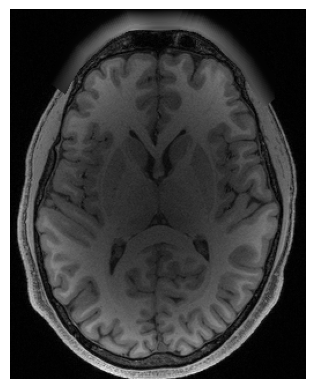
\includegraphics[width=\textwidth]{img/100206_T1.png}
        \caption{A T\textsubscript{1} weighted scan.\\$\text{\ac{tr}} = 2400.0$\\$\text{\ac{te}} = 2.14$}\label{fig:t1_t2_t1}
    \end{subfigure}
    ~
    \begin{subfigure}[t]{0.4\textwidth}
        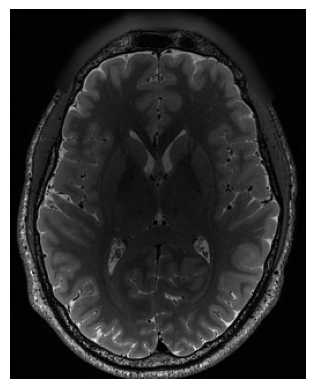
\includegraphics[width=\textwidth]{img/100206_T2.png}
        \caption{A T\textsubscript{2} weighted scan.\\$\text{\ac{tr}} = 3200.0$\\$\text{\ac{te}} = 565.0$}\label{fig:t1_t2_2}
    \end{subfigure}
    \caption{Two \ac{mri} scans of the same patient weighted differently. Both images have been created at a B\textsubscript{0} of \SI{3}{T}. Pixel values have been scaled to fill the entire available range. Note the difference in tissue color between weightings. These images have been adapted from data provided by the Human Connectome Project~\cite{human_connect}.}\label{fig:t1_t2}
\end{figure}

As T\textsubscript{2} usually sets in earlier than T\textsubscript{1}, each can be filtered out by a 
variation in scan parameters; \textit{\acf{te}} and \textit{\acf{tr}}. \ac{te} 
describes the time between the application of B\textsubscript{1} and the recording of a 
signal, while \ac{tr} refers to the time in-between pulses of B\textsubscript{1}. Due to
T\textsubscript{1}'s and T\textsubscript{2}'s difference (up to multiple seconds~\cite[p.~16]{medical_imaging})
their contribution to the overall signal are affected significantly differently.

% \; \: and \, are spaces in math mode
\begin{equation}\label{eq:tr_te}
    \textnormal{MR Signal} \propto \text{PD}\;\;\:\cdot\;\;\:\underbrace{(1-e^{-\frac{\text{TR}}{\text{T}_1}})}_{\text{T\textsubscript{1} Component}} \;\;\:\cdot \underbrace{e^{-\frac{\text{TE}}{\text{T}_2}}}_{\text{T\textsubscript{2} Component}}
\end{equation}

As shown in Equation.~\ref{eq:tr_te}~\cite[p.~26]{mri_handbook}, the proportion 
of influence to the signal of T\textsubscript{1} rises with \ac{tr}, while that of T\textsubscript{2} 
falls with a longer \ac{te}. By removing the other component's influence,
\iac{mri} scan can be \textit{T\textsubscript{1} weighted} or \textit{T\textsubscript{2} weighted} 
respectively~\cite{medical_imaging,introduction_to_particle_physics,mri_the_basics}.

\subsubsection{The NIfTI-1.1 Format}

A standardized representation of the data acquired through \ac{mri} facilitates
saving, transmitting and editing that data. One standard covering this use case is the
\textit{NIfTI-1.1} file format. Along with the voxel scan data, associated metadata
can be preserved using this format. Such metadata includes both metadata 
describing the image acquisition, e.g.~slice thicknesses and relation between
voxel and physical position, and added custom information about the preserved 
image data, such as annotations~\cite{nifti-1}.

\subsection{Classification}\label{sec:intro_classification}

The discipline of machine learning regularly revolves around the prediction of 
certain events or properties. Such predictions are made using records of already
well-known events, and the factors leading up to them. For example, using 
historical weather data, a model can make guesses about tomorrow's average
temperature. In turn, current temperatures, when compared to that same 
historical data, can also be used to determine the current season. When trying to
continue the list of daily temperatures, a model is trying to continue a 
stream of continuous values by a continuous value. Although tomorrow's 
temperature may fall into a certain limited range, the possibilities to choose
from are still infinite; this model is performing \textit{regression}.
Meanwhile, the model predicting seasons uses its available information to 
generate a result that is part of a predetermined limited set, such as 
\enquote{Spring}, \enquote{Summer}, \enquote{Fall} or \enquote{Winter}; this 
model is performing \textit{classification}. % Ask about "Formally, image classification can be interpreted as a mapping from ... to ..." ...
Formally, classification can be interpreted as the mapping from one domain into 
the label domain; a domain consisting of a subset of $ \mathbb{N} $\footnote{Note, that multidimensional classification is possible and not covered by this description. As the classification used here maps onto a single dimension, that use-case is treated here.}. In this case,
classification maps the image domain, in the shape of \ac{mri} scans to two 
labels $\in \mathbb{N} $, such as $\{0, 1\}$, representing either non-\acs{pcr}
or \ac{pcr} of the patient. 

As the prediction of a patient's
\ac{pcr} is based on a classification model, this section is a short overview
of its underlying concepts. Classification is the aim of a multitude of models. These include \acp{svm}, 
which try to separate classes by splitting features along multidimensional 
planes and decision trees, which use features to assemble multiple interlinked
\enquote{questions} that sort classes through their answers. Decision trees 
form the base of the classifier model used here.

\subsubsection{Decision Trees}

The structure of a decision tree follows that of the widely used data structure;
a collection of \textit{nodes}, all connected by \textit{edges} to, directly or 
through other nodes, a single \textit{root node}, where no edge creates a 
loop. In a decision tree, a root node represents the first question of that 
tree. This question can be answered using that node's edges; each edge pointing
away from a node contains an answer to the posed question. These edges then lead
to additional nodes, the \textit{children} of the node the edge originated from.
If this new node has edges pointing away from it, it contains an additional 
question. As edges lead in a single defined direction, that is, away from the 
root node, decision trees are \textit{directed trees}. Should a node be attached
only by edges pointing to it, this node is 
a \textit{leaf node}. When arriving at a leaf node, no further questions are 
raised. Instead, the content of the leaf node represents the final decision
gained by answering all questions leading up to it. For the case of 
classification this final decision would be the assignment to a class~\cite{tree_data_structure}.

% TODO: Refer to this
\begin{figure}[H]
    \centering
    \begin{tikzpicture}[every tree node/.style={draw}]
        \tikzset{level distance=60pt, sibling distance=25pt}

        \Tree [.{Year divisible by 4?} 
                \edge node[auto=right] {No};
                [.{Common Year} ]
                \edge node[auto=left] {Yes};
                [.{Year divisible by 100?} 
                    \edge node[auto=right] {No};
                    [.{Leap Year} ]
                    \edge node[auto=left] {Yes};
                    [.{Year divisible by 400?} 
                        \edge node[auto=right] {No};
                        [.{Common Year} ] 
                        \edge node[auto=left] {Yes};
                        [.{Leap Year} ]
                    ] 
                ] 
            ] 
                
    \end{tikzpicture}

    \caption{A simple decision tree, determining if a year is a leap year.}\label{fig:decision_tree}
\end{figure}

Such a decision tree is shown in Figure~\ref{fig:decision_tree}. The input for 
this tree would be a set of year numbers. Taking one of these numbers, its 
properties (or features) can be used to answer the question posed by the root 
node. Following the appropriate edge, and answering any following questions will
finally lead to a leaf node. The leaf node reached will contain the 
classification of the input; the answer whether the year number is a leap year.

\subsubsection{Constructing Decision Trees}

In some cases, the construction of a decision tree may seem obvious; nodes can 
be constructed to clearly separate classes and the resulting classification is
free of error. But as the size of datasets and the amount and complexity of 
their features rise, a clearly defined way of constructing decision trees is 
required. To determine along what quality to split a dataset, that is, through
which question to determine the further progression through the tree, every
possible new node must be evaluated through a common measure. This measure 
determines, which split is chosen to achieve the best overall performance for
the classification tree. One such measure, the \textit{purity} of a split will
be utilized here.
Purity describes how well a node, or its question, manages to split the dataset
along its classes. If, after one node, no part of the input is lumped together
with one of a different class, that node is completely pure. Inversely, the more
mixed between classes the output of a node is, the more impure that node is.
Pure nodes are generally preferred, as they lead to smaller, more effective 
trees. Sorting by purity, nodes are connected starting at the root and branching
out into branches and leaves. The tree stops growing when either perfect purity
is achieved, i.e.~the entire set is correctly classified, no nodes are left or
a predetermined maximum tree depth is reached~\cite{classification_and_regression_trees,gini_index_vs_information_gain,decision_tree_learning}.

\subsubsection{\aclp{rf}}

A decision tree can in theory be used to classify any amount of data utilizing
a feature vector of arbitrary length. Should a tree not achieve full purity, 
there will always be an error in classification. Inversely, if a decision tree
achieves a perfect classification rate, this may mean it is overfitted on its 
training set. This means, as that model fits its training set, and only its 
training set, perfectly, it manages classification on any additional datasets
considerably worse than non-overfitted models. Additionally, individual trees
tend to be unstable; a change in a single node affects all of its children.
Slight changes in the dataset, such as random noise, can strongly affect the
construction and outcomes of a 
tree~\cite{elements_of_statistical_learning,classification_and_regression_trees}.

To avoid this, a collection of trees, sometimes called a forest, can be used. By
taking random samples of the training set per tree, selecting a small random subset of 
available features at each node and using the best (most \enquote{pure}) parameter to split on, a group of decision trees are constructed. When 
classifying a member of the test set, that member passes through every tree, 
generating a prediction from each. Using those individual classifications, the
member is then assigned to the class that received the most \enquote{votes}, 
i.e.~the most chosen class by individual trees. This ensemble of randomly 
generated trees forming a forest is known as a \acf{rf} classifier~\cite{random_forests_article,random_forests_web}. 

The accuracy of a tree are measured during its construction by splitting off a
portion of all available cases. This portion is then used to test already 
constructed trees. Additionally, this enables the determination of individual
features' contribution to the final result. First, the reserved set is classified
using the constructed forest, counting correct votes for each case. Then, a 
single variable is swapped randomly between cases and they are classified again.
If performance suffers after swapping the variable, this variable contributes
strongly to the forest's performance, making it more 
important~\cite{random_forests_article,random_forests_web}. 

\subsubsection{Evaluation}

\acp{rf}, as with classifier models in general, can be evaluated using a set of
metrics. The two methods explored here are the \textit{confusion matrix} and 
the \textit{\acf{roc} curve}, using hold-out evaluation. Note, that although the evaluation of a model 
does not by itself have any influence on the performance of a model, it has a
strong influence on the perceived performance of a model. Depending on 
evaluation method, a model can be perceived to perform better or 
worse~\cite{evaluating_learning_algorithms}. The methods treated here were 
chosen because of their relatively common use in similar studies~\cite{multisite_rectal_radiomics,radiomics_analysis_pcr_rectal}. % TODO: Does this need a citation?

In the context of this thesis, all metrics described are calculated based
on the process of hold-out evaluation. This involves splitting an available 
dataset into two parts; a \textit{training set} and a \textit{testing set}.
The training is used in conjunction with known class labels to construct a 
classifier. The class labels are used to estimate and minimize the expected 
error rate of that classifier. Then, the testing set is passed to the model,
stripped of labels. By measuring its performance in classifying the testing set,
a model is evaluated~\cite{evaluating_learning_algorithms,fundamentals_of_machine_learning}.

The confusion matrix contains information about every classification. For $n$ 
classes in the dataset it forms an $n \times n$ matrix. In this matrix, the sum 
of all entries in row $i$ represents the amount of cases assigned to class $i$ 
by the classifier. Meanwhile, the sum of elements in row $j$ represents the 
number of elements that class $j$ actually contains. Every cell $ij$ in the 
matrix represents how many cases of class $j$ have been predicted to belong to 
class $i$. If $i = j$, cell $ij$ contains \textit{true} predictions. 
If $i \neq j$, all predictions in that cell are \textit{false}~\cite{evaluating_learning_algorithms}.

For a binary classification, such as \enquote{\ac{pcr} of a patient}, 
classifications can be separated into four distinct groups. If a prediction 
accurately assigns a label ($i = j$), that prediction is true; is the prediction 
positive (\enquote{the patient will recover}),
it is \iac{tp}, if not (\enquote{the patient will not recover}), it is \iac{tn}. In contrast, if the prediction 
fails ($i \neq j$), a positive assignment results in \iac{fp} (\enquote{the patient was expected to recover, but did not}), while a negative
prediction yields \iac{fn} (\enquote{the patient recovered, but was not expected to do so}).
These relations between predicted and actual outcomes are shown in Table~\ref{tbl:confusion_matrix}.

\begin{table}[h]
    \centering
    \begin{tabularx}{12cm}{Y!{\vrule width 1.5pt}Y|Y}
         & \textbf{Positive Prediction} & \textbf{Negative Prediction} \\\noalign{\hrule height 1.5pt}
        \textbf{Positive Case}  & \textit{\acf{tp}} & \acf{fn} \\ \hline
        \textbf{Negative Case} & \acf{fp} & \textit{\acf{tn}} \\
    \end{tabularx}\caption{A confusion matrix for binary classification. The vertical axis going from top left to bottom right represents correct classifications, written in \textit{italics}. Adapted from~\cite{evaluating_learning_algorithms}.}\label{tbl:confusion_matrix}
\end{table}

The total number of predictions in one of these groups reveals little about the
performance of a classifier. A high total count of \ac{tp} classifications may 
just as well stem from a large sample size as from a well constructed model.
For this reason, a \textit{\ac{tpr}} can be calculated. By setting in 
contrast the number of \ac{tp} predictions to that of positive cases in the dataset, the probability of a positive case being recognized as such is found. This
ratio, as shown in Equation~\ref{eq:true_positive_rate}, can be applied to any
group; by dividing the number of true assignments to a class by that of the 
members of that class, the rate of recognition of that class is
gained. The same can be calculated from false assignments, yielding the rate of
misclassification~\cite{evaluating_learning_algorithms,fundamentals_of_machine_learning}.

\begin{equation}
    \text{\acl{tp} Rate} = \frac{\text{\acl{tp} Predictions}}{\text{Positive Cases}} = \frac{\acs{tp}}{\acs{tp} + \acs{fn}}
    \label{eq:true_positive_rate}
\end{equation}

In the context of classification, two more metrics based on the confusion matrix
are used; \textit{sensitivity}, which equates to the \ac{tpr}, and 
\textit{specificity}, which represents the ratio of \ac{tn} predictions to the 
sum of \ac{fp} and \ac{tn} predictions, also known as the \ac{tnr}. Respectively, these measures describe
which portion of actually positive and actually negative cases were recognized 
as such. A composite metric of these scores is the \textit{balanced accuracy}, 
defined as in Equation~\ref{eq:ba}~\cite{evaluating_learning_algorithms,fundamentals_of_machine_learning,balanced_accuracy_and_posterior}.
By combining information about both the recognition of positive and negative 
cases, it provides an overview of the model's total accuracy. This is especially
useful, if the dataset is unbalanced, i.e.~if one label is more abundant than 
the other. If a dataset consisted of \SI{90}{\percent} positive cases, and only
\SI{10}{\percent} negative cases, a model labelling every case as 
\enquote{positive} would achieve both a \enquote{normal} accuracy of 0.9 
and \iac{tpr} of 1.0. By giving \ac{tnr} an equal 
weight in the total score, the accuracy (now balanced) would sink to 0.5.

\begin{equation}
    \text{Balanced Accuracy} = \frac{\frac{\text{\acl{tp} Predictions}}{\text{Positive Cases}} + \frac{\text{\acl{tn} Predictions}}{\text{Negative Cases}}}{2} = \frac{\acs{tpr} + \acs{tnr}}{2}
    \label{eq:ba}
\end{equation}

Another metric for model performance can be constructed by seeking an ideal 
balance in the trade-off between the \ac{tpr} and the \ac{fpr}. This is 
possible, because \iac{rf} classifier does not solely put any case into one of two 
classes. Due to its assembly of voting trees, \iac{rf} classifier can return
the (estimated) probability of a case being positive. By moving the threshold
for the minimum probability to classify a case as \enquote{true}, the 
sensitivity of a model can be raised or lowered. If the model would accept all cases as 
true (a threshold of 0.0), it would achieve \iac{tpr} of 1.0, while
raising its \ac{fpr} to 1.0. As the \ac{fpr} is directly correlated to the 
\ac{tnr}, this being $\text{\ac{tnr}} = 1.0 - \text{\ac{fpr}}$, this significantly lowers the balanced accuracy. 
To achieve the best possible trade-off between these two metrics, \iac{roc} 
curve can be constructed, by plotting the \ac{tpr} against the \ac{fpr}. One such 
curve is shown in Figure~\ref{fig:roc}, representing the results of differing 
classifier thresholds.


% Adapted from https://tex.stackexchange.com/questions/464887/drawing-roc-curve-analysis
\newcommand{\roccolor}{purple}
\begin{figure}[H]
    \centering

    \begin{tikzpicture}
        \begin{axis}[
        title={\acl{roc} Curve},
        xlabel={\acl{fpr}},
        ylabel={\acl{tpr}}, 
        xmin=0.0, 
        xmax=1.0,
        ymin=0.0,
        ymax=1.0,
        ]

        % To shade between
        \path [name path=xaxis]
            (0,0.5) --
            (1,0.50) --
            (1,1);

        \addplot [name path=roc, \roccolor] coordinates {
            (0, 0)
            (0, 0.15)
            (0.1, 0.15)
            (0.1, 0.25)
            (0.2, 0.25)
            (0.2, 0.6)
            (0.3, 0.6)
            (0.3, 0.75)
            (0.5, 0.75)
            (0.5, 0.85)
            (0.8, 0.85)
            (0.8, 0.95)
            (0.95, 0.95)
            (0.95, 1)
            (1, 1)
        };

        % \addplot [
        % thick,
        % color=blue,
        % fill=blue, 
        % fill opacity=0.5
        % ]
        % fill between[
        %     of=roc and xaxis,
        %     soft clip={domain=0:1},
        % ];

        
        \addplot [red, dashed] coordinates {
            (0, 0)
            (1, 1)
        };


        \end{axis}
\end{tikzpicture}
\caption{The \ac{roc} curve of a fictional classifier. The solid \roccolor{} line shows the performance of the model, while the dashed red line shows the result of random guesses. The larger the area below the curve, i.e.~the farther the model is away from random guessing, the bigger the \acs{auc} and the performance of the model. A curve running below the center line would suggest swapped labels.}\label{fig:roc}
\end{figure}


The \ac{roc} curve shows the ability of a model to recognize a positive case as
such, against the probability of misidentifying a negative case as positive.
If these probabilities are equal, the model is guessing randomly. The total 
performance of the model at the full range of thresholds can be calculated by
the deviation from random guesses, i.e.~the center line. \Iac{roc} curve 
usually runs above this line, as the opposite would suggest swapped labels. 
Therefore, measuring all space below the curve yields a new metric, the 
so-called \acf{auc}~\cite{evaluating_learning_algorithms,fundamentals_of_machine_learning}.
